In the next two tables can be consulted the schedule for the assignments to be completed during the project's implementation (Table \ref{table:requirements}) and the description of each assignment type (Table \ref{table:activityType}).
\begin{center}
	\begin{table}[H]
		\caption{Requirements}
		\makebox[\textwidth][c]{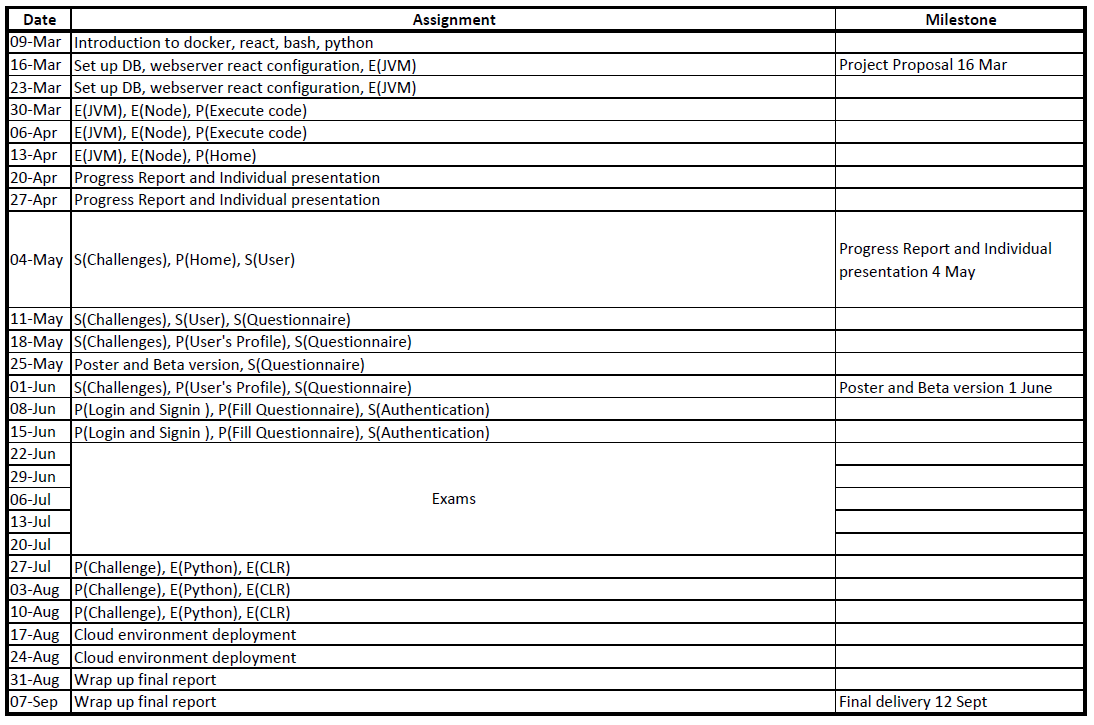
\includegraphics[width=1.2\textwidth]{./imgs/requisitiosV2.PNG}}%
  		%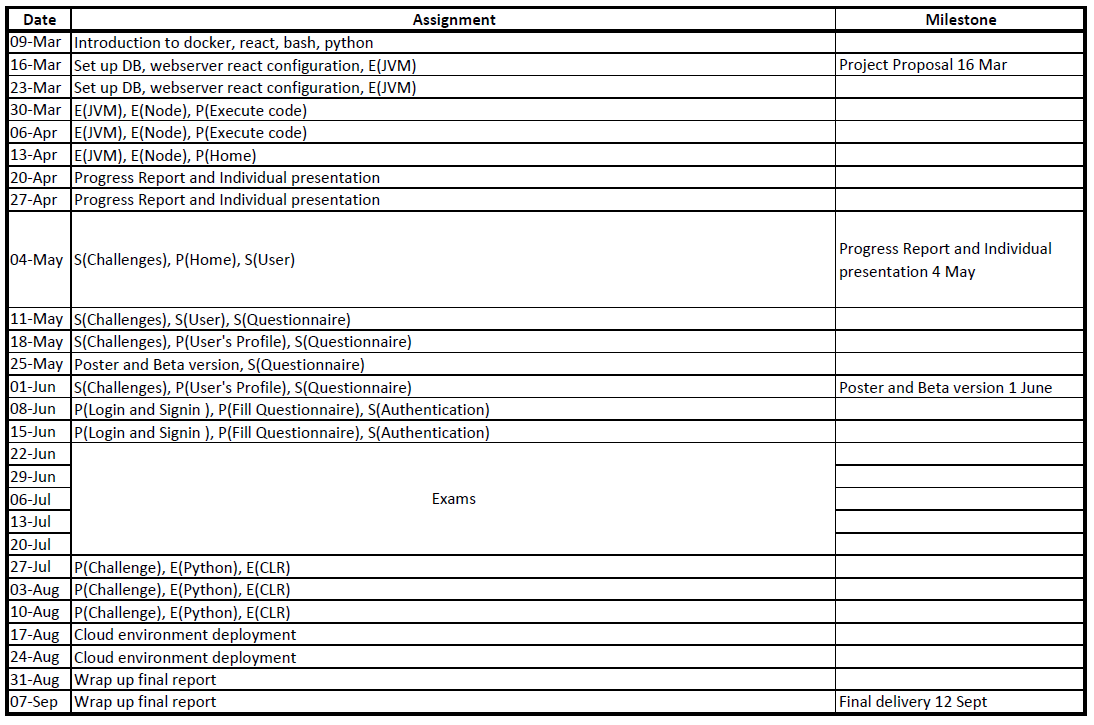
\includegraphics[scale=0.5]{./imgs/requisitiosV2.PNG}
  		
  		\label{table:requirements}
	\end{table}
\end{center}

\begin{center}
	\begin{table}[H]
		\caption{Assignment Types}
		\makebox[\textwidth][c]{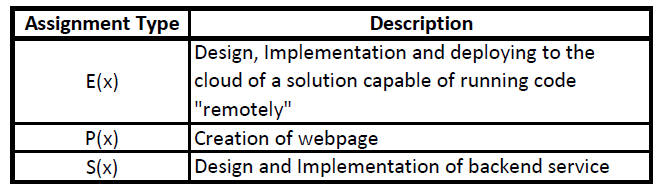
\includegraphics[width=0.6\textwidth]{./imgs/activityType.PNG}}%
  		%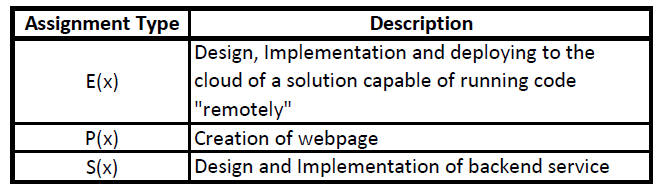
\includegraphics[scale=0.5]{./imgs/activityType.PNG}
  		\label{table:activityType}
	\end{table}
\end{center}